%% LyX 2.3.8 created this file.  For more info, see http://www.lyx.org/.
%% Do not edit unless you really know what you are doing.
\documentclass[spanish,a4paper, 10pt, onecolumn, journal]{ieeeconf}
\usepackage[T1]{fontenc}
\usepackage[utf8]{inputenc}
\setcounter{secnumdepth}{3}
\setcounter{tocdepth}{3}

\makeatletter
%%%%%%%%%%%%%%%%%%%%%%%%%%%%%% User specified LaTeX commands.
\overrideIEEEmargins
\usepackage{fancyhdr}
\usepackage{lastpage}
\usepackage{graphicx}
\usepackage{amsmath}
\usepackage{amssymb} % Para símbolos matemáticos adicionales
\usepackage{adjustbox}
\usepackage{cleveref}
\usepackage{array}

\newcommand{\defeq}{\mathrel{\mathop:}=}
\newcolumntype{C}[1]{>{\centering\arraybackslash}m{#1}}
\renewcommand{\arraystretch}{1.5} % Ajusta este valor para más o menos espacio entre filas
\usepackage[prepend]{epstopdf}
\graphicspath{{imagenes/}}

% Configuración del encabezado y el pie de página
\pagestyle{fancy}
\fancyhf{}

% Encabezado
\fancyhead[L]{UNCuyo -- Ing. Mecatrónica \\ Mendoza - Argentina}
\fancyhead[C]{\textbf{311 -- AUTOMÁTICA Y MÁQUINAS ELÉCTRICAS \\ PROYECTO GLOBAL INTEGRADOR}}
\fancyhead[R]{Año: 2024 \\ Alumnos: Borquez y Escobar\\Fecha: 06/06/2024}

% Pie de página
\fancyfoot[C]{Página \thepage\ de \pageref{LastPage}} % Muestra "Página x de xx"


\fancypagestyle{plain}{
  \fancyhf{}  % Limpiar todos los encabezados y pies de página
  \fancyhead[L]{UNCuyo -- Ing. Mecatrónica \\ Mendoza - Argentina}
  \fancyhead[C]{\textbf{311 -- AUTOMÁTICA Y MÁQUINAS ELÉCTRICAS \\ PROYECTO GLOBAL INTEGRADOR}}
  \fancyhead[R]{Año: 2024 \\ Alumnos: Borquez y Escobar\\Fecha: 06/06/2024}fancyhead[R]{Mi Encabezado Derecho}   % Encabezado derecho
  \fancyfoot[C]{Página \thepage\ de \pageref{LastPage}} % Muestra "Página x de xx"
}

% Línea en la parte superior del encabezado
\renewcommand{\headrulewidth}{0.4pt}

% Línea en la parte inferior del pie de página
\renewcommand{\footrulewidth}{0.4pt}

\makeatother

\usepackage{babel}
\addto\shorthandsspanish{\spanishdeactivate{~<>}}

\begin{document}
\title{\textbf{Proyecto Global Integrador: Control de Accionamiento de CA
con Motor Sincrónico de Imanes Permanentes}}
\author{Borquez Juan y Escobar Matías}
\maketitle
\begin{abstract}
En
\end{abstract}

\section{INTRODUCCIÓN}

El estudio que se presenta en este documento trata sobre el modelado,
simulación, diseño y análisis de desempeño de un Sistema de Control
Automático de Posición y Movimiento para un Accionamiento electromecánico
de 4 cuadrantes, compuesto por: una máquina eléctrica de corriente
alterna (CA) trifásica sincrónica con excitación por imanes permanentes
(PMSM), alimentada por inversor trifásico desde fuente de corriente
continua (CC); un reductor de velocidad de engranajes planetarios
de salida hacia la carga mecánica; realimentación con 1 sensor de
posición en el eje del motor, más 3 sensores de corriente instantánea
de fases en la salida del inversor trifásico y 1 sensor de temperatura
del bobinado de estator.

\section{PRESENTACIÓN DEL PROBLEMA}

El problema bajo estudio se encuentra bien detallado en la guía de
referencia key-1, por lo que en esta sección se indican solo los
aspectos más relevantes de cada una de las partes del problema junto
con las ecuaciones que modelan cada parte del sistema.

\subsection{Carga Mecánica}

La aplicación se trata del control de movimiento de 1 eje (descentralizado)
para articulación de brazo manipulador robótico elemental de un grado
de libertad (1 g.d.l.) rotacional de eje horizontal sometido a la
acción de la aceleración de gravedad (péndulo rígido actuado), con
eje de rotación fijo a base en sistema de referencia inercial con
parámetros equivalentes variables según sea la carga útil transportada
en el extremo.

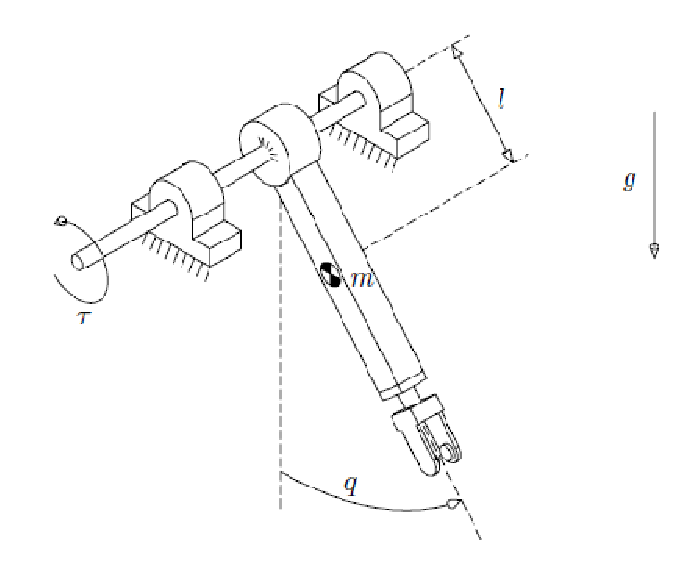
\includegraphics[width=\columnwidth]{1-Brazo.eps} 
\begin{thebibliography}{G. O. Young, ``Synthetic structure of industrial plastics (Book style with paper title and editor),'' 	in Plastics, 2nd ed. vol. 3, J. Peters, Ed.  New York: McGraw-Hill, 1964, pp. 15--64.}
\bibitem[R. Kelly et al, Control of Robot Manipulators in Joint Space. Springer, 2005. (Example and Figure 2.2).]{key-1}

\bibitem[G. O. Young, ``Synthetic structure of industrial plastics (Book style with paper title and editor),'' 	in Plastics, 2nd ed. vol. 3, J. Peters, Ed.  New York: McGraw-Hill, 1964, pp. 15--64.]{key-2}

\bibitem[ P. Krause et al, Analysis of Electric Machinery and Drive Systems, 3rd Ed.. IEEE-Wiley, 2013.]{key-3}

\bibitem[B. Smith, ``An approach to graphs of linear forms (Unpublished work style),'' unpublished.]{key-4}

\bibitem[E. H. Miller, ``A note on reflector arrays (Periodical styleÑAccepted for publication),'' IEEE Trans. Antennas Propagat., to be publised.]{key-5}

\bibitem[J. Wang, ``Fundamentals of erbium-doped fiber amplifiers arrays (Periodical styleÑSubmitted for publication),'' IEEE J. Quantum Electron., submitted for publication.]{key-6}

\end{thebibliography}

\end{document}
